\chapter{Protótipos de monitores da qualidade do ar desenvolvidos}\label{apendix: hw-prototypes}

Foram desenvolvidos dois protótipos para o monitoramento da qualidade do ar ilustrados na Figura \ref{fig:monitoring-prototypes} do Capítulo \ref{cap:clean-initiative}. Eles foram baseados na plataforma Arduino Mega 2560, que utiliza o microcontrolador ATMega2560 da Microchip. Um deles foi projetado para medição fixa em um local, e o outro para monitoramento de forma móvel. Este último, além de prover a informação temporal associada a cada leitura de concentração de poluente, inclui a localização onde a medição foi tomada. Os dispositivos foram projetados para a medição de poluentes regulados na Resolução CONAMA No. 491/2018, sendo eles: \acrshort{co}, \acrshort{no2}, \acrshort{so2} e \acrshort{o3}. Além desses gases, a versão fixa também inclui um sensor de sulfeto de hidrogênio ($H_2S$). 

A Figura \ref{fig:diagrama-sistemas} mostra diagramas com os módulos de \textit{hardware} que compõem os sistemas de medição fixo e móvel, sem incluir o processo de transporte dos gases. A versão fixa do sistema de monitoramento (Figura \ref{fig:estrutura-fixo}) utiliza seis sensores da empresa Alphasense sensíveis aos gases \acrshort{co}, \acrshort{no2}, \acrshort{so2}, \acrshort{o3} e $H_2S$. Além destes, também estão instalados quatro sensores da empresa SPEC, sensíveis aos mesmos poluentes com exeção do $H_2S$. A conexão entre a plataforma Arduino Mega e os sensores SPEC é realizada pela porta serial UART2 do microcontrolador através de um barramento RS-485. Já a leitura dos sensores da Alphasense é realizada pelas entradas analógicas AI0 – AI11 do microcontrolador.

\begin{figure}[h]
    \centering
    \caption{Diagrama de blocos dos sistemas fixo (a) e móvel (b)}
    \begin{subfigure}{0.495\textwidth}
        \centering
        \includegraphics[width=\textwidth]{aftertext/Protótipos desenvolvidos/Figuras/Estrutura versão fixa.png}
        \caption{}
        \label{fig:estrutura-fixo}
    \end{subfigure}
    \hfill
    \begin{subfigure}{0.495\textwidth}
        \centering
        \includegraphics[width=\textwidth]{aftertext/Protótipos desenvolvidos/Figuras/Estrutura versão móvel.png}
        \caption{}
        \label{fig:estrutura-mov}
    \end{subfigure}
    \label{fig:diagrama-sistemas}
    \fonte{Desenvolvido pelo autor (2023)}
\end{figure}

A versão móvel (Figura \ref{fig:estrutura-mov}) utiliza apenas sensores da SPEC para a medição de gases. Os modelos SPEC utilizados nesta versão são os mesmos que na versão fixa, e utilizam a mesma configuração para se comunicar de forma serial com o Arduino Mega. Um diferencial desta versão com relação à fixa, além de não utilizar sensores Alphasense, é a inclusão de um módulo GPS para georreferenciar as medições dos poluentes. O módulo utilizado é o GY-NEO6MV2 que se comunica com o microcontrolador através da UART1.

Além dos dispositivos mencionados acima, cada unidade de monitoramento inclui um módulo ESP8266 ESP-01 conectado à porta serial UART3 do Arduino, para comunicação Wi-Fi. Ambas unidades utilizam também um módulo de cartão micro SD para o armazenamento dos dados e um módulo de Relógio de Tempo Real (RTC) para manter a informação de data e hora. Outros periféricos como sensor de pressão, monitor LCD ou atuadores para controlar o transporte dos gases, podem ser adicionados através do barramento I2C em versões futuras.

Os módulos que compõem ambos sistemas de medição funcionam com tensões de alimentação tanto de 3.3 V como 5 V. Para fornecer esses níveis de voltagem foi utilizado um módulo-fonte que utiliza dois reguladores AMS1117. Um dos reguladores fornece uma saída 3.3 V e o outro 5 V. Ambos reguladores conseguem fornecer até 1 A de corrente de saída. O módulo-fonte possui dois canais de entrada de tensão. Um canal possui um conector Jack P4 para tensões entre 9 – 15 V, enquanto o outro possui um conector USB fêmea para fornecer uma tensão de 5 V.

O sistema fixo é alimentado com uma tensão de 12 V, aplicada no conector Jack P2 do módulo-fonte. Os 12 V de tensão podem ser provenientes de uma fonte conectada à rede elétrica, ou de um controlador solar conectado a um painel solar e uma bateria de 12 V. Já o sistema móvel pode ser alimentado por qualquer carregador de bateria portátil com saída em formato USB de 5 V e mínimo 2 A de corrente.

As seções seguintes descrevem cada um dos blocos que compõem os protótipos desenvolvidos.

\section{Transporte de gases}
\begin{table}
    \centering
    \caption{Especificações técnicas dos ventiladores utilizados no equipamento fixo e móvel}
    \begin{tabularx}{0.95\textwidth}[h]{
         >{\raggedright\arraybackslash}X
         >{\raggedright\arraybackslash}X 
         >{\raggedright\arraybackslash}X }
         \hline
        \textbf{Características} & \textbf{Versão fixa} & \textbf{Versão móvel} \\ [0.5ex] 
       \hline
        Descrição & Ventilador cooler 40mm 12VDC & Ventilador cooler 40mm 5VDC \\ 
        \hline
        Marca & GC & GDT \\ 
        \hline
        Tamanho & 40 x A: 40 x C: 10mm & L: 40 x A: 40 x C: 10mm \\
        \hline
        Corrente nominal & 80 ± 10\% mA & 140 ± 10\% mA \\
        \hline
        Tensão nominal & 12 V & Entre 5 e 7V \\
        \hline
        Ruído & 16 ± 10\% dBA & 16 ± 10\% dBA \\
        \hline
        Velocidade rotação & 5000 ± 10\% RPM & 7000 ± 20\% RPM \\
        \hline
        Fluxo de ar & 4.2 CFM & 6.12 CFM \\
        \hline
        Peso & 12 g & 14 g \\
        \hline
        Consumo potência & 1.2 W & 0.8 W \\
        \hline
        Vida útil & 35000 hr & 50000 hr \\
        \hline
    \end{tabularx}
    \label{tab:esp-ventiladores}
\end{table}

A etapa de transporte de gases é tida como a entrada do sistema. Sua função é capturar amostras do ar no ambiente e direcioná-las para o conjunto de sensores. Nos protótipos desenvolvidos, esta etapa é formada por dois ventiladores de corrente direta e uma câmara de gases. Os ventiladores conduzem o ar desde o ambiente de monitoramento até o interior da câmara. Esta última, por outro lado, consiste em um volume que retém o ar amostrado. No interior dela, os sensores são expostos às porções de ar coletadas para extrair informação de alguns poluentes que podem estar nelas contidos.

As configurações dos ventiladores variam de acordo com a versão do protótipo que os contêm. A versão fixa utiliza ventiladores com tensão nominal de 12 V, e a instalação mecânica deles foi realizada em série para conseguir maior pressão no fluxo do ar. Os ventiladores utilizados na versão móvel, por outro lado, têm uma tensão nominal de 5 V e foram colocados em paralelo. Suas características principais estão dispostas na Tabela \ref{tab:esp-ventiladores}.

\section{Sensoriamento}
A etapa de sensoriamento consiste em um arranjo de sensores de gases eletroquímicos e os circuitos de condicionamento analógico ou interfaces digitais correspondentes. Os sensores utilizados nos protótipos variam da versão fixa para a móvel, mas de forma geral foram instalados sensores do tipo \textit{screen-printed} fabricados pela SPEC Sensors LLC., e sensores da série B4 da Alphasense Ltd. Os dispositivos de transdução escolhidos são sensíveis aos poluentes regulados na Resolução CONAMA No. 491/2018: \acrshort{co}, \acrshort{no2}, \acrshort{so2}, \acrshort{o3}. Além desses gases, foi monitorado também o sulfeto de hidrogênio ($H_2S$) com um sensor de Alphasense. A modo de ilustração, a Figura \ref{fig:sensors} mostra os modelos SPEC DGS-CO 968-034 e Alphasense O3-B4, utilizados na medição de \acrshort{co} e \acrshort{o3}.

\begin{figure}[h]
    \centering
    \caption{Sensores dos fabricantes a) SPEC e b) Alphasense}
    \begin{subfigure}{0.495\textwidth}
        \centering
        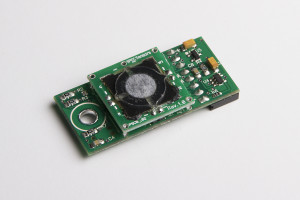
\includegraphics[width=\textwidth]{aftertext/Protótipos desenvolvidos/Figuras/SPEC IoT.jpg}
        \caption{}
        \label{fig:spec-iot}
    \end{subfigure}
    \hfill
    \begin{subfigure}{0.495\textwidth}
        \centering
        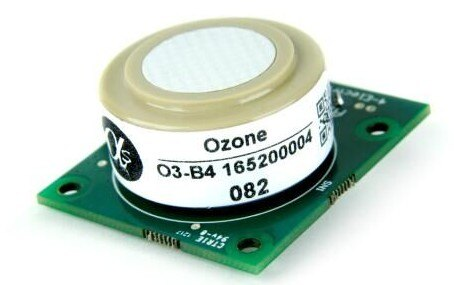
\includegraphics[width=\textwidth]{aftertext/Protótipos desenvolvidos/Figuras/Alphasense w ISB.jpg}
        \caption{}
        \label{fig:alpha-isb}
    \end{subfigure}
    \label{fig:sensors}
\end{figure}

A versão fixa dos instrumentos desenvolvidos contém arranjos de sensores das empresas SPEC e Alphasense. Já o equipamento móvel dispõe apenas de um arranjo de sensores da SPEC Sensors. A seguir são descritas características dos sensores de cada fabricante.

\subsection{Sensores SPEC}
Os sensores da SPEC possuem a configuração característica de três eletrodos (de trabalho, contador e de referência). A sigla SPEC provêm do inglês Screen-Printed Electro-Chemical, que é a tecnologia de manufatura utilizada por esse fabricante para produzir seus sensores. Essa tecnologia possibilita fabricar sensores de gases eletroquímicos de alta performance em um encapsulamento fino e de um custo menor que os encapsulamentos mais volumosos, utilizados tradicionalmente para fabricar sensores eletroquímicos \cite{SPECSensors2016SPECConsiderations}. A Figura \ref{fig:spec-iot} mostra o sensor SPEC DGS-CO 968-034, utilizado na medição de monóxido de carbono, em sua placa de condicionamento. A Tabela \ref{tab:esp-SPEC} resume as principais características dos sensores que foram utilizados dessa empresa. 

\begin{table}[b]
    \centering
    \caption{Especificações técnicas dos sensores SPEC}
    \label{tab:esp-SPEC}
    \begin{tabularx}{0.98\textwidth}[h]{
         >{\raggedright\arraybackslash}X
         >{\raggedleft\arraybackslash}X 
         >{\raggedleft\arraybackslash}X
         >{\raggedleft\arraybackslash}X 
         >{\raggedleft\arraybackslash}X }
         \hline
        \textit{Características} & $CO$ & $NO_2$ & $SO_2$ & $O_3$ \\
        \hline
        Modelo & DGS-CO 968-034 & DGS-NO2 968-043 & DGS-SO2 968-038 & DGS-O3 968-042 \\ 
        \hline
        Intervalo de medição & 0 - 1000 ppm & 0 - 5 ppm & 0 - 20 ppm & 0 - 5 ppm \\
        \hline
        Resolução & 100 ppb & 20 ppb & 50 ppb & 20 ppb \\
        \hline
        Tensão nominal & 3.3 V & 3.3 V & 3.3 V & 3.3 V \\
        \hline
        Consumo de potência & 12 mW & 14 mW & 12 mW & 14 mW \\
        \hline
        Tempo de resposta* & < 30 s & < 30 s & < 30 s & < 30 s \\
        \hline
        Temperatura de operação & -20 – 40 ºC & -20 – 40 ºC & -20 – 40 ºC & -20 – 40 ºC \\
        \hline
        Umidade relativa de operação & 15 – 95 \% & 15 – 95 \% & 15 – 95 \% & 15 – 95 \% \\
        \hline
    \end{tabularx}
\end{table}

\subsection{Sensores Alphasense}
Os sensores da série B4, da Alphasense, utilizam, além dos três eletrodos característicos do princípio de medição eletroquímico, um quarto eletrodo chamado de Eletrodo Auxiliar. Sua função é gerar uma corrente com um valor de intensidade muito próximo ao valor da corrente de fundo do zero (zero background current). Dessa forma é possível compensar a saída dos sensores do efeito desta corrente de zero ou de linha base. A Tabela \ref{tab:esp-ALPHA} resume as principais características dos sensores que foram utilizados desse fabricante.

\begin{table}
    \centering
    \caption{Especificações técnicas dos sensores Alphasense}
    \begin{tabularx}{0.98\textwidth}[h]{
        >{\raggedright\arraybackslash}X
        >{\raggedleft\arraybackslash}X
        >{\raggedleft\arraybackslash}X
        >{\raggedleft\arraybackslash}X
        >{\raggedleft\arraybackslash}X
        >{\raggedleft\arraybackslash}X }
        \hline
        \textit{Características} & $CO$ & $NO_2$ & $SO_2$ & $O_3$ & $H_2S$ \\
        \hline
        Modelo & CO-B4 & NO2-B43F & SO2-B4 & OX-B431 & H2S-B4 \\ 
        \hline
        Intervalo de medição (ppm) & 0 - 1000 & 0 - 20 & 0 - 100 & 0 - 20 & 0 - 100 \\
        \hline
        Resolução (ppb) & 4 & 15 & 5 & 15 & 1 \\
        \hline
        Tempo de resposta (s)* & < 30 & < 80 & < 60 &  < 80 & < 60 \\
        \hline
        Temperatura de operação (ºC) & -30 – 50 & -30 – 40 & -30 – 50 & -30 – 40 & -30 – 50 \\
        \hline
        Umidade relativa de operação (\%) & 15 – 90 & 15 – 85 & 15 – 90 & 15 – 85 & 15 – 90 \\
        \hline
    \end{tabularx}
    \label{tab:esp-ALPHA}
\end{table}

\section{Condicionamento}
A configuração mais utilizada nos circuitos de condicionamento dos sensores eletroquímicos é o potenciostato. Este circuito controla o potencial aplicado ao eletrodo de trabalho e converte a corrente desse eletrodo em um valor de tensão.

A empresa Alphasense disponibiliza para os sensores da série B4 uma placa de condicionamento chamada de \textit{Individual Sensor Board} (ISB). Esta placa transforma o sinal de corrente de saída do sensor em um sinal de tensão proporcional ao valor de concentração do gás. A SPEC Sensors, por sua vez, disponibiliza uma placa com um microcontrolador dedicado, que condiciona a saída do transdutor e entrega o dado de concentração mediante uma interface digital serial.

\subsection{Interface de condicionamento dos sensores Alphasense: A Placa de Sensoriamento Individual (ISB)}
As placas ISB da Alphasense possuem circuitos de potenciostato compatíveis com a família de sensores B4, de quatro eletrodos. Nesses circuitos, tanto o eletrodo de trabalho quanto o auxiliar possuem etapas de amplificação equivalentes. As tensões de saída destes dois eletrodos são disponibilizados em um conector Molex de 6 vías junto com os canais para a alimentação da placa. A tensão de alimentação das placas ISB pode ser entre 3.5 e 6.4 VDC; nos protótipos desenvolvidos foi utilizada uma tensão de 5 VDC.

O diagrama ilustrado na Figura \ref{fig:interface-alpha} apresenta as conexões realizadas entre a plataforma Arduino e os sensores da Alphasense através das placas ISB. Percebe-se que cada conjunto composto por um sensor e seu respectivo circuito de condicionamento, ocupa duas entradas analógicas do microcontrolador; uma entrada para o eletrodo auxiliar (AE) e outra para o eletrodo de trabalho (WE). No total foram utilizadas os canais analógicos A0 – A11.

\subsection{Interface de condicionamento dos sensores SPEC}
Assim como os sensores da Alphasense, os sensores da empresa SPEC também utilizam um circuito de condicionamento de potenciostato. Na mesma placa de condicionamento, a SPEC tem incorporado um microcontrolador dedicado e sensores de temperatura e umidade. O microcontrolador converte o valor de tensão de saída do potenciostato em um valor digital de concentração de gás, e realiza uma compensação, por software, dos efeitos da temperatura e a umidade na medição.

O kit de condicionamento SPEC funciona como uma camada de abstração no que diz respeito ao tratamento e condicionamento das informações, garantindo uma fácil integração com os sistemas de monitoramento. O dispositivo disponibiliza as informações de data e hora, o valor de concentração em ppm/ppb e as leituras de temperatura e umidade através de uma interface serial UART. De igual modo, podem ser realizadas operações como calibração, ajuste de zero e span, configuração dos sensores, e seleção de modo de operação de baixo consumo de energia, através de uma biblioteca com comandos pré definidos \cite{SPECSensors2017Digital968-045}.

\begin{figure}[t]
    \centering
    \caption{Interface entre os sensores e o microcontrolador Arduino. a) Alphasense, b) SPEC}
    \begin{subfigure}{0.39\textwidth}
        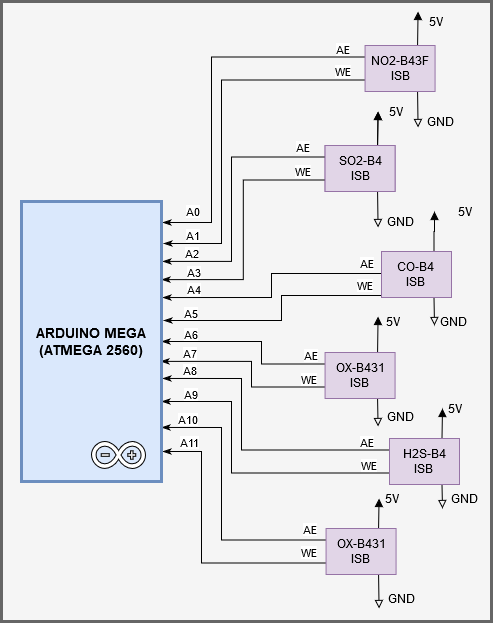
\includegraphics[width=\textwidth]{aftertext/Protótipos desenvolvidos/Figuras/Interface com sensores Alphasense.png}
        \caption{}
        \label{fig:interface-alpha}
    \end{subfigure}
    \hfill
    \begin{subfigure}{0.6\textwidth}
        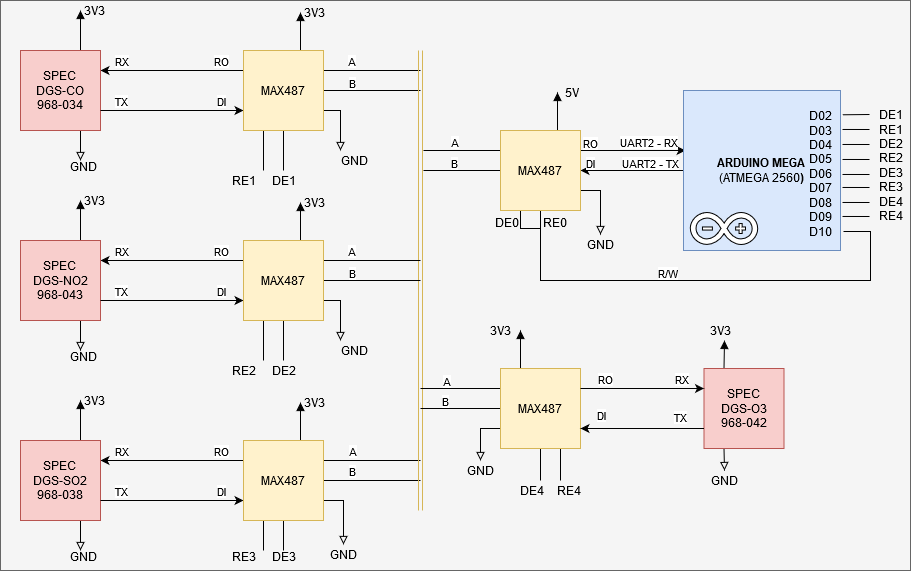
\includegraphics[width=\textwidth]{aftertext/Protótipos desenvolvidos/Figuras/Interface com sensores SPEC.png}
        \caption{}
        \label{fig:interface-spec}
    \end{subfigure}
    \hfill
    \label{fig:circuitos-interface}
    \fonte{Desenvolvido pelo autor (2023)}
\end{figure}

A Figura \ref{fig:interface-spec} apresenta um diagrama da conexão do arranjo de sensores da SPEC à plataforma Arduino Mega. Os sensores e o microcontrolador ATMega2560 são acoplados a um barramento RS-485 mediante o transceptor MAX487. Esse transceptor provê uma interface entre os meios de comunicação serial UART e RS-485. O barramento RS-485 consiste basicamente em dois fios A e B que fornecem o meio físico para a transmissão de níveis de tensão que representam os dados seriais enviados pelos diferentes dispositivos. O nível do sinal transmitido através do barramento é determinado pela tensão diferencial entre os conectores A e B, independentemente da voltagem de alimentação dos dispositivos conectados. Como mostra a figura, os transceptores dos sensores são alimentados com uma tensão de 3.3 VDC, enquanto o transceptor do Arduino é alimentado pelo mesmo sinal de 5 VDC que o microcontrolador.

É possível conectar múltiplos dispositivos a um mesmo barramento RS-485 (máximo até 128), sendo necessária a ação de um controlador que determine quem acessa o meio físico a cada instante, para evitar colisões. O microcontrolador ATMega2560 realiza essa função através das saídas digitais D02 – D10. Esses sinais digitais controlam o estado das entradas $RE_i$ e $DE_i$ de cada MAX487, a fim de habilitar/desabilitar cada transceptor para operações de escrita/leitura.

\section{Microcontrolador}
A etapa de processamento engloba todas as funcionalidades de controle, temporização, geolocalização, aquisição dos dados dos sensores, comunicação e armazenamento dos dados. Todas essas funções são gerenciadas pelo microcontrolador ATMega2560 da Microchip, embarcado na plataforma Arduino Mega 2560. Mais detalhes sobre o firmware desenvolvido para o controle da etapa de processamento são abordados no Apêndice \ref{appendix: firmware}. A continuação descrevem-se cada um dos módulos que compõem esta etapa.

\subsection{Armazenamento dos dados}
Para o armazenamento dos dados foi utilizado um módulo para fazer leitura e escrita diretamente em um cartão micro SD. A comunicação é feita por meio de uma interface SPI, conforme se mostra na Figura \ref{fig:interface-SD}. O nível de sinal é de 3.3V, mas o módulo possui divisores de tensão nos seus pinos que possibilitam uma ligação direta com placas que trabalham com 5 V, como o Arduino. O módulo é alimentado com uma tensão de 5 V, e suporta cartões Micro SD e Micro SDHC de alta velocidade.

\begin{figure}[h]
    \centering
    \caption{Interface entre o módulo cartão micro SD e o microcontrolador}
    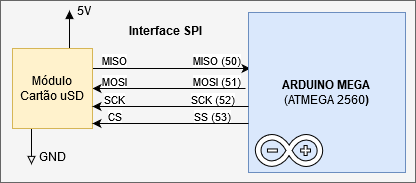
\includegraphics[width=0.7\textwidth]{aftertext/Protótipos desenvolvidos/Figuras/Interface com micro SD.png}
    \label{fig:interface-SD}
    \fonte{Desenvolvido pelo autor (2023)}
\end{figure}

\subsection{Controle de data e hora e geolocalização}
Para manter o controle da data e hora do sistema fixo, e assim acrescentar informação temporal às leituras de gases, foi utilizado o módulo de Relógio de Tempo Real (RTC) DS1307. O DS1307 é um relógio/calendário de baixo consumo de potência que utiliza um barramento $I^2C$ bidirecional para a transferência de dados desde (e para) o microcontrolador. O relógio/calendário provê informação de segundos, minutos, horas, dia, mês e ano, incluindo ajuste automático de ano bissexto e de meses com menos de 31 dias. O DS1307 é alimentado por uma tensão de 5 V, e também possui um circuito que detecta falhas de energia e automaticamente aciona a alimentação através de uma bateria. Quando isso sucede, o relógio/calendário mantém a contagem do tempo em um modo de baixo consumo (consumo de corrente menor que 500 nA), estendendo o tempo de vida útil da bateria. A Figura \ref{fig:interface-rtc} mostra como é realizada sua conexão ao microcontrolador no sistema desenvolvido.

\begin{figure}[h]
    \centering
    \caption{Interface entre o microcontrolador e os módulos a) RTC e b) GPS}
    \begin{subfigure}{0.49\textwidth}
        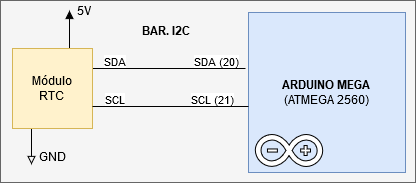
\includegraphics[width=\textwidth]{aftertext/Protótipos desenvolvidos/Figuras/Interface com RTC.png}
        \caption{}
        \label{fig:interface-rtc}
    \end{subfigure}
    \hfill
    \begin{subfigure}{0.49\textwidth}
        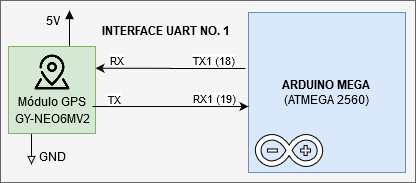
\includegraphics[width=\textwidth]{aftertext/Protótipos desenvolvidos/Figuras/Interface com GPS.png}
        \caption{}
        \label{fig:interface-gps}
    \end{subfigure}
    \hfill
    \label{fig:interface-RTC_GPS}
    \fonte{Desenvolvido pelo autor (2023)}
\end{figure}

Na versão móvel, ambos os controles da data e hora e geolocalização são realizados por um mesmo dispositivo GPS, o módulo NEO6MV2. O NEO6M é um receptor GPS de baixo consumo de potência e pequenas dimensões que o tornam uma opção interessante para dispositivos móveis. O módulo possui uma antena integrada, com precisão de aproximadamente 5 metros, e tecnologia para supressão de congestionamentos na comunicação e interferências. A conexão entre o módulo e a plataforma Arduino é realizada através de um barramento serial UART a uma taxa de transferência padrão de 9600 bauds (Figura \ref{fig:interface-gps}). Ele pode ser alimentado com uma tensão de 3.3 ou 5 V e seu consumo de corrente em pleno funcionamento chega a 45 mA. Seus pinos de entrada são compatíveis com níveis de tensão TTL e suportam tensões tanto de 5 como de 3.3 V, independentemente da tensão de alimentação.

\subsection{Comunicação Wi-Fi}
Para a comunicação Wi-Fi é utilizado o módulo ESP-01. Esse módulo incorpora o sistema integrado em um único chip (SoC, System on Chip) ESP8266EX, da empresa Espressif, e uma antena embarcada com ganho de potência de 3dBi, garantindo um alcance de até 90 metros em espaços abertos. O SoC ESP8266EX integra um processador de 32 bits, o Tensilica L106, que implementa os protocolos TCP/IP e o 802.11 b/g/n WLAN MAC. Ele possui como vantagens um baixo consumo de energia atrelado a uma velocidade de clock de 80 MHz. Sua memória RAM, disponível em aplicações em que o sistema está configurado como estação é de aproximadamente 36 kB. O módulo ESP-01 disponibiliza, para armazenar o programa de usuário, uma memória FLASH de 1MB externa que pode ser acessada por um barramento SPI. O módulo disponibiliza quatro portas digitais que são utilizadas principalmente para programar a FLASH de usuário e uma porta serial UART.

\begin{figure}[h]
    \centering
    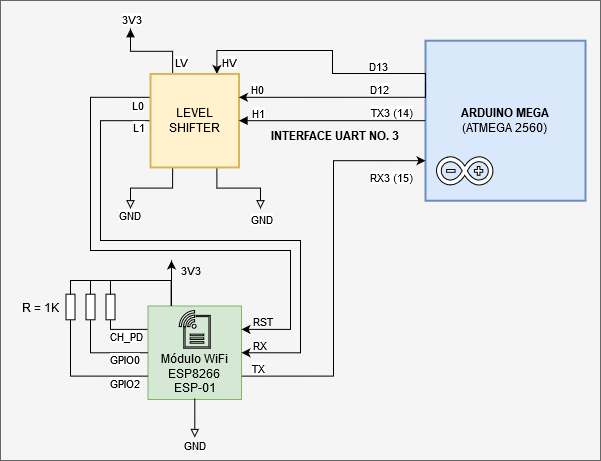
\includegraphics[width=0.6\textwidth]{aftertext/Protótipos desenvolvidos/Figuras/Interface com ESP8266.png}
    \caption{Interface entre o microcontrolador e o módulo de comunicação Wi-Fi}
    \label{fig:interface-esp}
    \fonte{Desenvolvido pelo autor}
\end{figure}

A Figura \ref{fig:interface-esp} apresenta as conexões realizadas entre o ESP-01 e a plataforma Arduino. O módulo opera com uma tensão de 3.3 V, por esse motivo é utilizado um circuito intermediário, um elevador de nível (level shifter) para converter os níveis de tensão de 5 V para 3.3 V, e vice-versa. O pino CH\_PD corresponde ao chip enable do ESP-01 e deve ser conectado a um resistor de \textit{pull-up} de 1 kΩ, assim como as entradas GPIO0 e GPIO2. Essas entradas são utilizadas para configurar o ESP8266 em modo gravação (para gravar o programa de usuário) ou modo estação. A figura mostra a configuração do modo estação, com ambas entradas conectadas à 3.3 V por meio de resistores de \textit{pull-up} de 1 kΩ. O pino de entrada RST tem como função reiniciar o módulo. Como esse pino é “ativo baixo”, cada vez que uma tensão de 0 V for aplicada nessa porta o módulo será reiniciado. No circuito desenvolvido, o Arduino pode reiniciar o ESP8266 através da saída digital D12. Já a saída D13 do microcontrolador Arduino é encarregada de manter uma tensão de referência de 5 V no elevador de nível para possibilitar a conversão dos níveis de tensão.

\section{Montagem do protótipo fixo}

A seguir descreve-se brevemente a montagem e interligação dos elementos de hardware que compõem o protótipo de medição fixa. A Figura \ref{fig:fixed-prototype-field-inst} mostra o protótipo de monitor fixo instalado em campo. O quadro externo é a caixa ambiental modelo Atlantic 352 00 da Cemar \& Legrand com nível de proteção IP66.

\begin{figure}[h]
    \centering
    \caption{Instalação em campo do protótipo fixo}
    \includegraphics[width=0.4\linewidth]{aftertext/Protótipos desenvolvidos/Figuras/Instalacão fixo.jpg}
    \label{fig:fixed-prototype-field-inst}
\end{figure}

As Figuras \ref{fig:fixed-prototype} e \ref{fig:fixed-prototype-int} mostram o módulo de sensoriamento, que é a parte fundamental de todo o sistema. Nele são contidos todos os elementos que compõem o sistema e que foram descritos anteriormente.

\begin{figure}[h]
    \centering
    \caption{Vista interior do protótipo fixo}
    \begin{subfigure}{0.495\textwidth}
        \centering
        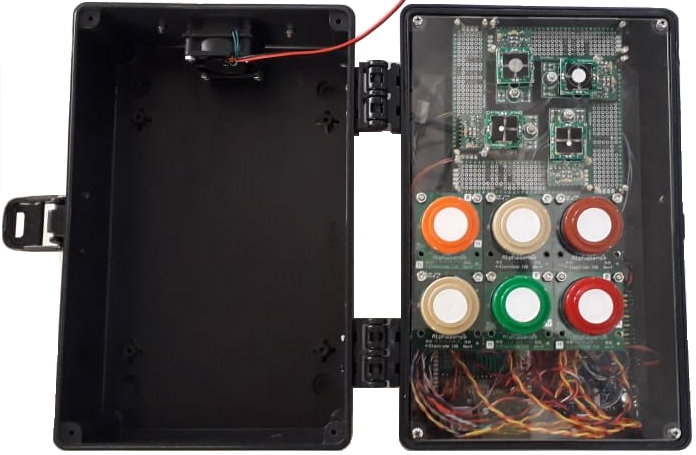
\includegraphics[width=\textwidth]{aftertext/Protótipos desenvolvidos/Figuras/clean-fixed-prototype.png}
        \caption{Vista superior}
        \label{fig:fixed-prototype}
    \end{subfigure}
    \hfill
    \begin{subfigure}{0.495\textwidth}
        \centering
        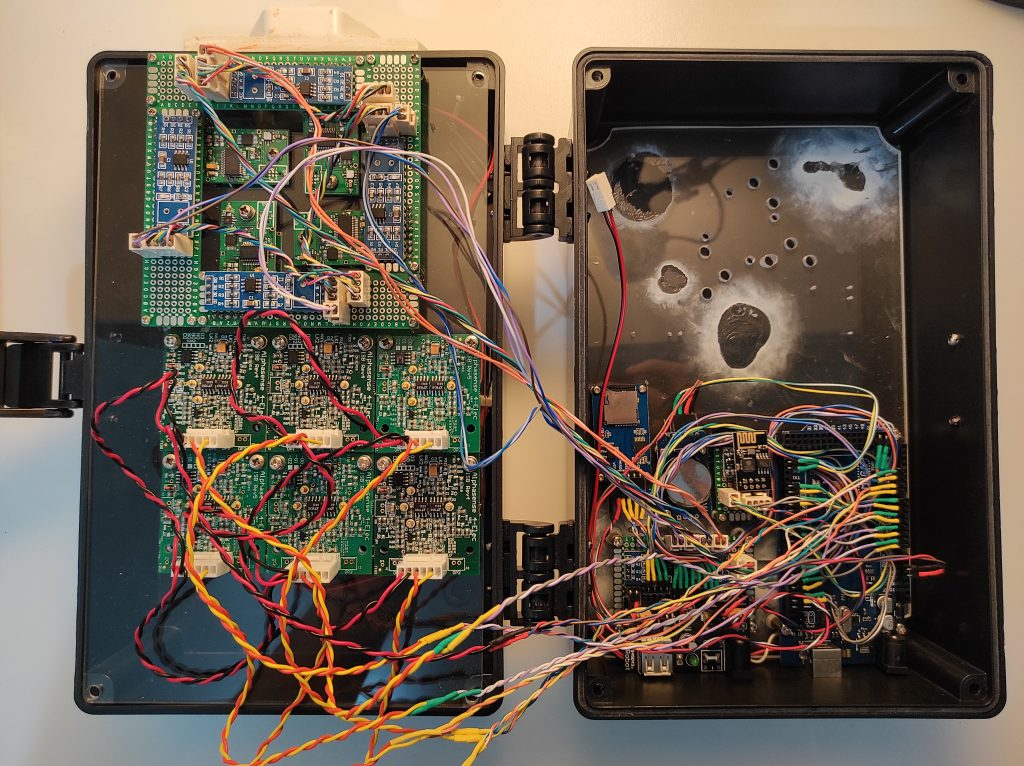
\includegraphics[width=\textwidth]{aftertext/Protótipos desenvolvidos/Figuras/clean-fixed-prototype-internal.jpg}
        \caption{Vista inferior}
        \label{fig:fixed-prototype-int}
    \end{subfigure}
    \label{fig:prototypes}
\end{figure}

Um sistema de transporte de gases, composto por duas ventoinhas de 12VDC, coleta amostras do ar ambiente para dentro da câmara. A entrada é composta por uma flange de 50 mm de diâmetro (que serve para acoplar a câmara no restante do sistema de transporte de gases) e um filtro de tecido. As dimensões das ventoinhas são 40x40mm, e foram fixadas com quatro parafusos M2x30mm com porca e arruela. Dentro do volume da câmara, as superfícies dos sensores de gás interagem com os componentes gasosos e produzem um sinal de resposta proporcional à concentração do gás. A Tabela \ref{tab:list-of-sensors} resume os sensores e placas de condicionamento que foram utilizados nesssa versão do equipamento.

\begin{table}[h]
    \caption{Lista de sensores utilizados no protótipo fixo}
    \label{tab:list-of-sensors}
    \centering
    \begin{tabularx}{0.95\textwidth}[h]{
         >{\raggedright\hsize=.10\hsize\arraybackslash}X
         >{\raggedright\hsize=.40\hsize\arraybackslash}X 
         >{\raggedright\arraybackslash}X
         >{\raggedright\hsize=.30\hsize\arraybackslash}X }
        \hline
        \textbf{Qtd.} & \textbf{Ítem} & \textbf{Descrição} & \textbf{Fabricante}\\
        \hline
        1 & CO-B4 & Sensor de \acrshort{co} & Alphasense \\
        \hline
		1 & H2S-B4 & Sensor de \acrshort{h2s} & Alphasense \\
        \hline
		1 & SO2-B4 & Sensor de \acrshort{so2} & Alphasense \\
        \hline
        1 & NO-B4 & Sensor de \acrshort{no} & Alphasense \\
        \hline
        1 & NO2-B43F & Sensor de \acrshort{no2} & Alphasense \\
        \hline
        1 & OX-B431 & Sensor de \acrshort{o3} & Alphasense \\
        \hline
        1 & NH3-B1 & Sensor de \acrshort{nh3} & Alphasense \\
        \hline
        3 & CO/H2S/SO2 4-electrodes ISB & Placa de condicionamento para sensores da série B4 que medem \acrshort{co}, \acrshort{h2s} e \acrshort{so2} & Alphasense \\
        \hline
        1 & NO 4-electrodes ISB & Placa de condicionamento para sensores da série B4 que medem \acrshort{no} & Alphasense \\
        \hline
        1 & NO2/O3 4-electrodes ISB & Placa de condicionamento para sensores da série B4 que medem \acrshort{no2} e \acrshort{o3} & Alphasense \\
        \hline
        1 & NH3 4-electrodes ISB & Placa de condicionamento para sensores da série B4 que medem \acrshort{nh3} & Alphasense \\
        \hline
        1 & DGS-O3-968-042\_9-6-17 & Sensor de \acrshort{o3} para \acrshort{iot} & SPEC Sensors \\
        \hline
        1 & DGS-SO2-968-038 & Sensor de \acrshort{so2} para \acrshort{iot} & SPEC Sensors \\
        \hline
        1 & DGS-NO2-968-043-9-6-17 & Sensor de \acrshort{no2} para \acrshort{iot} & SPEC Sensors \\
        \hline
        1 & DGS-CO-968-034 & Sensor de \acrshort{co} para \acrshort{iot} & SPEC Sensors \\
        \hline
    \end{tabularx}
\end{table}

Uma placa de acrílico foi utilizada para fixar os sensores de maneira correta e isolar o \textit{hardware} do fluxo de ar. As conexões elétricas para levar os sinais de saída dos sensores até o Arduino foram feitas com fios de seção 0,2mm², soldando “\textit{headers}” nas pontas e isolando-as corretamente com duto termorretrátil. As Figuras \ref{fig:alphasense-power-supply} e \ref{fig:alphasense-connections} ilustram respectivamente diagramas de conexão da alimentação elétrica e dos eletrodos dos sensores ao Arduino.

\begin{figure}[h]
    \centering
    \caption{Diagrama de conexões do conjunto de sensores Alphasense}
    \begin{subfigure}{0.495\textwidth}
        \centering
        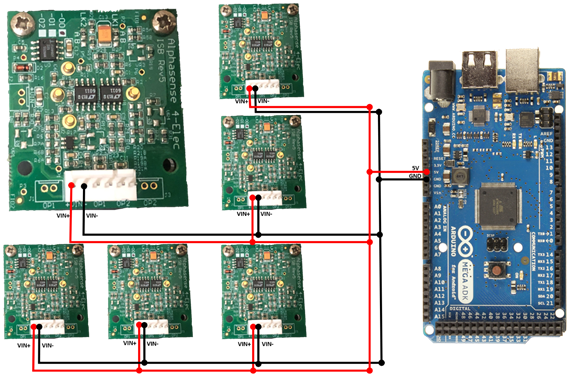
\includegraphics[width=\textwidth]{aftertext/Protótipos desenvolvidos/Figuras/Alimentação Alphasense.png}
        \caption{Alimentação elétrica}
        \label{fig:alphasense-power-supply}
    \end{subfigure}
    \hfill
    \begin{subfigure}{0.495\textwidth}
        \centering
        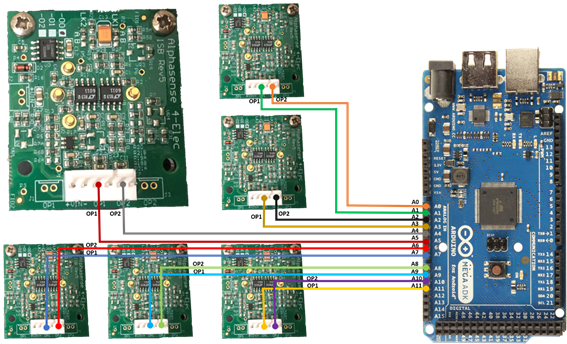
\includegraphics[width=\textwidth]{aftertext/Protótipos desenvolvidos/Figuras/Conexões Alphasense.png}
        \caption{Conexão dos eletrodos}
        \label{fig:alphasense-connections}
    \end{subfigure}
\end{figure}

A fixação dos sensores \textit{SPEC} na placa de acrílico mencionada anteriormente foi feita através de placas de prototipagem confeccionadas artesanalmente. Nas placas foram soldados “\textit{headers}” fêmeas encima dos quais os sensores foram montados. Nas placas também foram instalados os transceptores MAX487 que criam o barramento RS-485 para a conexão serial com o microcontrolador da placa Arduino. As placas são conectadas ao barramento através de fios e conectores do tipo MOLEX. As placas de prototipagem com os sensores foram fixadas diretamente à placa de acrílico com espaçadores M2.

Após a montagem do conjunto de sensores e prefixação dos componentes eletrônicos da câmara de medição, foi realizada a ligação elétrica de alimentação e comunicação de todos os componentes envolvidos no sistema. O diagrama de alimentação é mostrado na Figura \ref{fig:fixed-modules-power-supply}. Vale salientar que a alimentação da placa Arduino foi feita diretamente com 12V com fios soldados no conector P2 de entrada. Já a conexão do restante dos módulos com a placa Arduino é ilustrada na Figura \ref{fig:fixed-modules-connections}.

\begin{figure}[h]
    \centering
    \caption{Diagrama de conexões do conjunto de sensores Alphasense}
    \begin{subfigure}{0.495\textwidth}
        \centering
        \includegraphics[width=\textwidth]{aftertext/Protótipos desenvolvidos/Figuras/alimentação_fixo.png}
        \caption{Alimentação dos módulos do protótipo}
        \label{fig:fixed-modules-power-supply}
    \end{subfigure}
    \hfill
    \begin{subfigure}{0.495\textwidth}
        \centering
        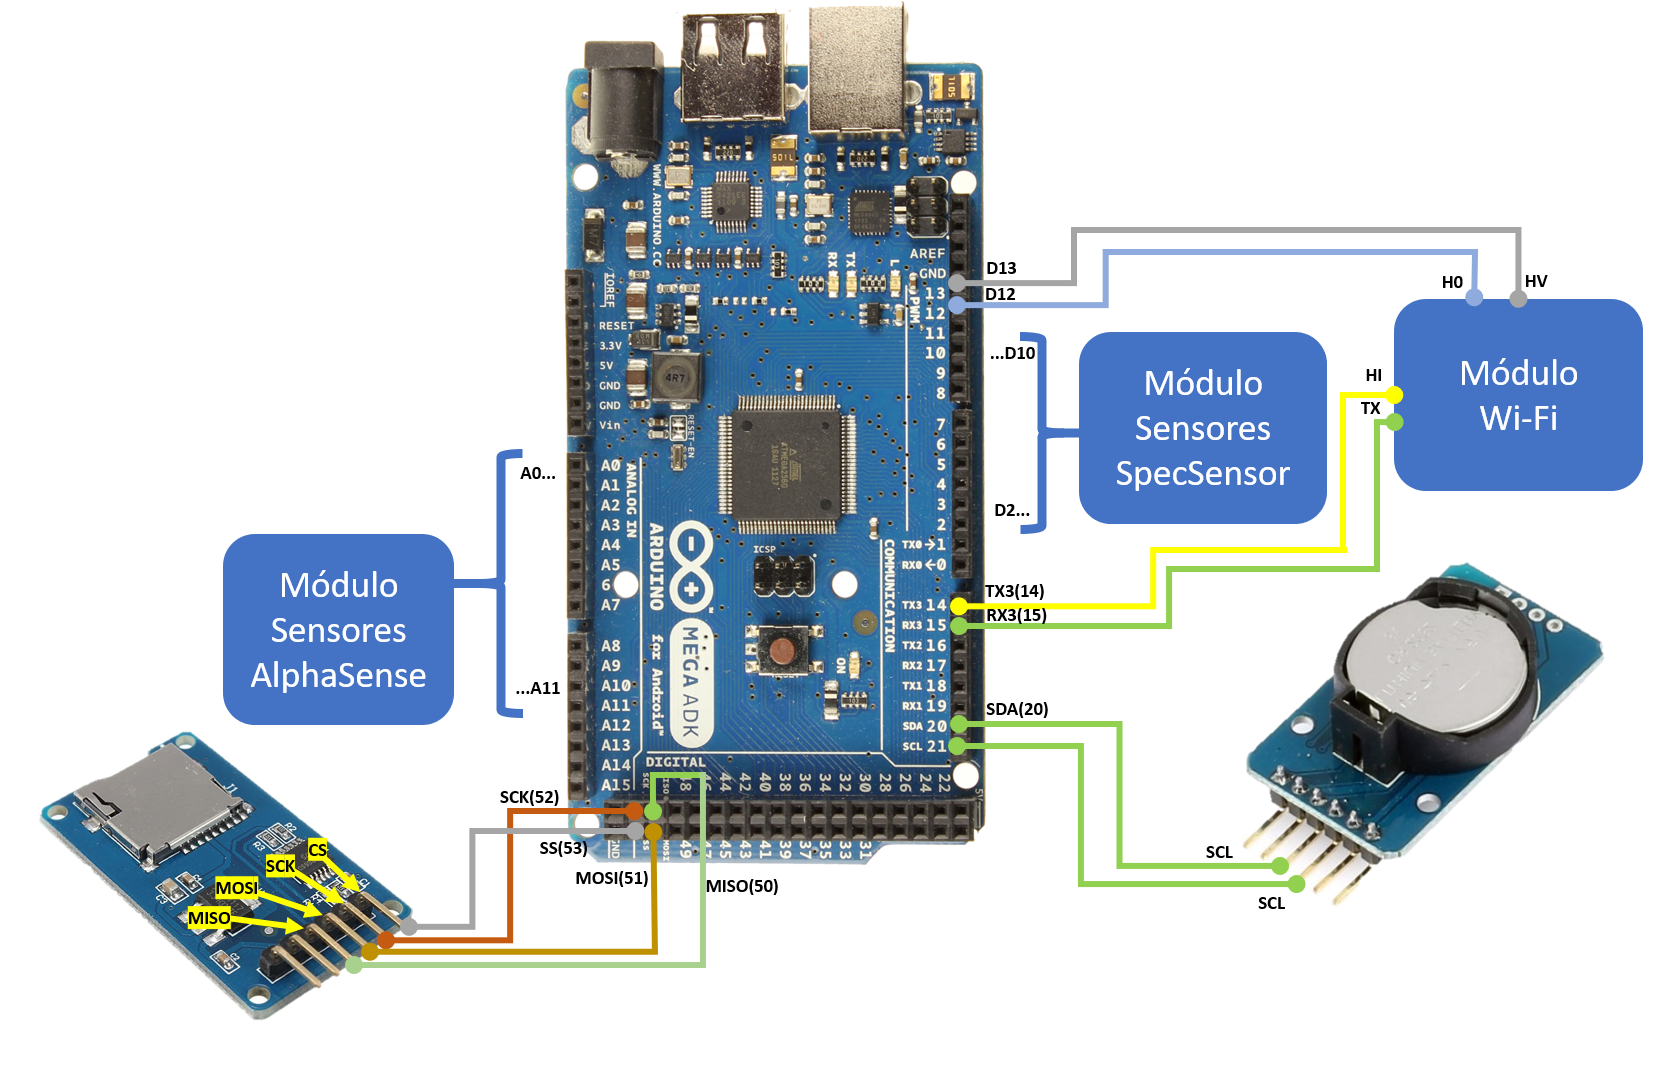
\includegraphics[width=\textwidth]{aftertext/Protótipos desenvolvidos/Figuras/comunicacao_fixo.png}
        \caption{Conexão dos módulos do protótipo}
        \label{fig:fixed-modules-connections}
    \end{subfigure}
\end{figure}

\section{Montagem do protótipo móvel}

O equipamento mede poluentes da legislação ambiental brasileira \cite{BRASIL.MINISTERIODOMEIOAMBIENTEMMA.ConselhoNacionaldoMeioAmbienteCONAMA2018ResolucaoAr.} que são: \acrshort{co}, \acrshort{no2}, \acrshort{so2}, \acrshort{o3} e \acrshort{h2s}. Para isso utiliza um conjunto de quatro sensores do fabricante SPEC Sensor que contemplam a medição desse poluentes. O controle da estapa de monitoramento, armazenamento e envio de dados é baseado na plataforma Arduino Mega 2560, que utiliza o microcontrolador ATMega2560 da Microchip. Para operar com sucesso, o sistema inclui: módulo Wi-Fi, módulo de cartão SD, módulo GPS e indicadores LED operacionais.